% !TeX spellcheck = da_DK
% Setup document class.
%  This will always be the beamer class, but depending on the use of notes,
%  it can be annotated with the option [notes] or  [notes=only], depending
%  on whether notes should be included, or should be the only thing in
%  the document.
\documentclass[xcolor=table]{beamer}

% Setup theme.
%\usetheme[
%%% options passed to the outer theme
%    progressstyle=fixedCircCnt,   %either fixedCircCnt, movCircCnt, or corner
%    rotationcw,          % change the rotation direction from counter-clockwise to clockwise
%    shownavsym          % show the navigation symbols
]{AAUsimple}

\usetheme[
%%% options passed to the outer theme
%    hidetitle,           % hide the (short) title in the sidebar
%    hideauthor,          % hide the (short) author in the sidebar
%    hideinstitute,       % hide the (short) institute in the bottom of the sidebar
%    shownavsym,          % show the navigation symbols
%    width=2cm,           % width of the sidebar (default is 2 cm)
    hideothersubsections,% hide all subsections but the subsections in the current section
%    hideallsubsections,  % hide all subsections
    left               % right of left position of sidebar (default is right)
%%% options passed to the color theme
%    lightheaderbg,       % use a light header background
  ]{AAUsidebar}



% Import preamble
%%% Initial things %%%
% Increase number of dimen registers
\usepackage{etex}
% Fix various issues with LaTeX2e
\usepackage{fixltx2e}
% Font package
\usepackage{fourier}


%%% Translations and character encodings %%%
% Enable use of several characters, including æ, ø and å
\usepackage[utf8]{inputenc}
% Danish language
\usepackage[danish]{babel}
% Use PostScript fonts instead of bitmap ones. Also does other stuff.
\usepackage[T1]{fontenc}
% Various LaTeX symbols
\usepackage{latexsym}
% Wider selection of colours
\usepackage{xcolor}
% Improved element justification
\usepackage{ragged2e}
% Font improvements
\usepackage{fix-cm}
% Enables various forms of lines, like double-underlining (\uuline{})
\usepackage{ulem}
% Sets the tolerance for distance between words, determining when to hyphenate.
\pretolerance=2500


%%% Figures and tables (Floats) %%%
% Enable multi-rows and -columns
\usepackage{multirow}
\usepackage{multicol}
% Double, horizontal lines
\usepackage{hhline}
% Enables coloured tables
\usepackage{colortbl}
% Prettier tables
\usepackage{booktabs}


%%% Mathematic formulas %%%
% AMS math
\usepackage{amsmath}
\usepackage{amssymb}
% Extra fonts (for math, I think)
\usepackage{stmaryrd}
% Access text symbols
\usepackage{textcomp}
% Extend AMS
\usepackage{mathtools}
\usepackage{cancel}


%%% Graphics %%%
% Various image-commands
\usepackage{eso-pic}
% Use JPEG and PNG images
\usepackage{graphicx}

%%% Code listing %%%
\usepackage{color}
\definecolor{bluekeywords}{rgb}{0.13,0.13,1}
\definecolor{greencomments}{rgb}{0,0.5,0}
\definecolor{redstrings}{rgb}{0.9,0,0}

\usepackage{courier}

\usepackage{listings}

\lstset{language=[Sharp]C,
  captionpos=b,            
  columns=fixed,     
  numbers=left,
  numberstyle=\tiny,
  showspaces=false,
  showtabs=false,
  breaklines=true,
  inputencoding=utf8,
  showstringspaces=false,
  breakatwhitespace=true,
  escapeinside={(*@}{@*)},
  commentstyle=\color{greencomments},
  keywordstyle=\color{bluekeywords},
  stringstyle=\color{redstrings},
  basicstyle=\ttfamily\small,
}

\lstdefinestyle{make}{tabsize=4}


%%% References, bibtex and URLs %%%
% Post URLs. Allows breaking at hyphens to help avoid long links.
\usepackage{url}
% Better cross references
\usepackage[danish]{varioref}
% Define a new 'leo' style for URL package, that will use a smaller font
\makeatletter
\def\url@leostyle{%
  \@ifundefined{selectfont}{\def\UrlFont{\sf}}{\def\UrlFont{\small\ttfamily}}
}
\makeatother
% And of course, use this new style
\urlstyle{leo}

\hypersetup{pdfstartview={Fit}}
%%%%%%%%%%%%%%%%%%%%%%%%%%%%%%%%%%%%%%%%%%%%%%%%
%Flowchart
\usepackage{tikz}
\usetikzlibrary{shapes.geometric, arrows, positioning}
%%%%%%%%%%%%%%%%%%%%%%%%%%%%%%%%%%%%%%%%%%%%%%%%

% Additional settings for boxes
\setbeamercolor{headerCol}{fg=black,bg=lightgray}
\setbeamercolor{bodyCol}{fg=white,bg=gray}
\setbeamercovered{transparent=20}

% Define document stuff
\title[ProjectFood]{Udvikling af applikationer fra brugere til data, algoritmer og test og tilbage igen}
\subtitle[Eksamen]{Eksamen}
\author[DS304E14]{Gruppe DS304E14}
\date{26. januar 2015}

\institute[
%  {\includegraphics[scale=0.2]{aau_segl}}\\ %insert a company, department or university logo
Software (SW3)\\
Aalborg Universitet\\
Danmark
] % optional - is placed in the bottom of the sidebar on every slide
{% is placed on the title page
  Software (SW3)\\
  Aalborg Universitet\\
  Danmark
  
  %there must be an empty line above this line - otherwise some unwanted space is added between the university and the country (I do not know why;( )
}

% Specify a logo on the titlepage (you can specify additional logos an include them in 
% institute command below
\pgfdeclareimage[height=1.5cm]{titlepagelogo}{AAUgraphics/aau_logo_new} % placed on the title page
%\pgfdeclareimage[height=1.5cm]{titlepagelogo2}{graphics/aau_logo_new} % placed on the title page
\titlegraphic{% is placed on the bottom of the title page
  \pgfuseimage{titlepagelogo}
  %  \hspace{1cm}\pgfuseimage{titlepagelogo2}
}


\begin{document}

{\aauwavesbg
  \begin{frame}[plain,noframenumbering]
    \titlepage
  \end{frame}}

% ==================== SUBJECTS ======================
%\section{Introduktion}

\begin{frame}{Disposition}
\begin{itemize}
   \item Metode og Problemanalyse - Marc
   \item Systemanalyse - Mathias Corlin
   \item Udvikling - Troels
   \item Test af system - Søren
   \item Demonstration af system - Mathias Sass
   \item Reflektion over projekt - Morten
\end{itemize}
\end{frame}

\section{Metode og Problemanalyse}
\subsection{Metoder}
\begin{frame}{Metoder}
\begin{itemize}
   \item Udvikling
   \item Analyse
   %Ikke for at udelade DEB, men den er der ikke blevet lagt vægt på metoder derfra
   \item Informationssamling
\end{itemize}
\end{frame}

\subsection{Udvikling}
\begin{frame}{Udvikling}
\begin{itemize}
   \item Evolutionær
   \begin{itemize}
      \item Filosofi
      \item Alternativ - Konstruktion
   \end{itemize}
   \item Adaption af scrum
   \begin{itemize}
      \item Scrum i arbejdsmiljøet
      \item Scrum i projektet
      %Gruppens udbytte heraf
   \end{itemize}
\end{itemize}
\end{frame}

\subsection{Analyse}
\begin{frame}{Analyse}
\begin{itemize}
   \item OOA\&D
   \begin{itemize}
      \item Klassediagram
      \item Hændelsestabel
      \item Brugsmønstre
      %Corlin will mention dis in detailz
   \end{itemize}
   \item Formål %Hvorfor ikke bare starte med systemet?
   \item Udbytte %Hvordan dette også gør det lettere at oprette scrum taskts og user stories
\end{itemize}
\end{frame}

\subsection{Informationssamling}
\begin{frame}{Informationssamling}
\begin{itemize}
   \item Interviews i kontekst
   \item State of the art analyse
   \item Prototype interviews
\end{itemize}
\end{frame}

\subsection{Problemformulering}
\begin{frame}{Problemformulering}
\[
  \left[
  \begin{minipage}{\textwidth}
  \centering
  \begin{minipage}{0.96\textwidth}
  \textit{Hvordan designes og implementeres et system, i C\#, der kan give brugere lettere adgang til dagligvarebutikkernes tilbud integreret med indkøbslister og opskrifter imens det gøres mere overskueligt, at handle ind til aftensmad?}
  \end{minipage} 
  \end{minipage}                           
    \right]
\]
%Quote problemformulering - bliv enig på gruppen om hvordan quote skal sættes op
\end{frame}
\input{slides/corlin.tex}
\section{Udvikling af programmet}
	\begin{frame}{Udvikling af programmet}\framesubtitle{Indhold}
		 \begin{itemize}
		 	\item Arkitektur
		 	\item Funktionskomponenter
		 	\item Modellag
		 	\item Programmering
		 	\item Teknologier
		 	\item API
		 \end{itemize}
	\end{frame}
	\subsection{Arkitektur}
		\begin{frame}[t]{Arkitektur}\framesubtitle{MVC \& Komponenter}
			\begin{columns}[T]
				\begin{column}{.48\textwidth}
					\begin{itemize}
						\item Website
						\item Client--Server arkitektur
						\item MVC
						\begin{itemize}
							\item Model
							\item View
							\item Controller
						\end{itemize}
						\item Opdelt i funktionskomponenter
					\end{itemize}

				\end{column}
				\begin{column}{.48\textwidth}
					\begin{figure}
						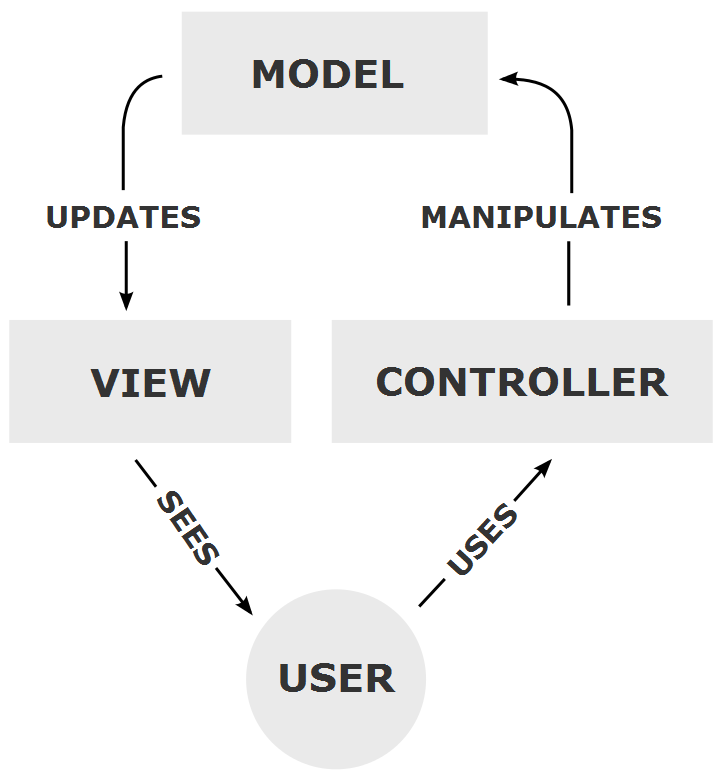
\includegraphics[width=1\textwidth]{images/MVC_2.png}
						\caption{MVC, figur af RegisFrey fra \url{wikipedia.org}}
					\end{figure}
				\end{column}
			\end{columns}
		\end{frame}
		
		\subsubsection{Funktionskomponenter}
		\begin{frame}[t]{Arkitektur}\framesubtitle{Funktionskomponenter}
			\begin{itemize}
				\item Funktionskomponenters adgange og afhængighedder
				\item Rækkefølge af komponenters implementering
			\end{itemize}
			%Topologisk sortering -> omvend reækkefølge -> implementer
			%Bruger > Tilbud > Indkøbsliste > Overvågning > Opskrift
			\vspace{-5pt}
			\begin{figure}[h!]
				\centering
				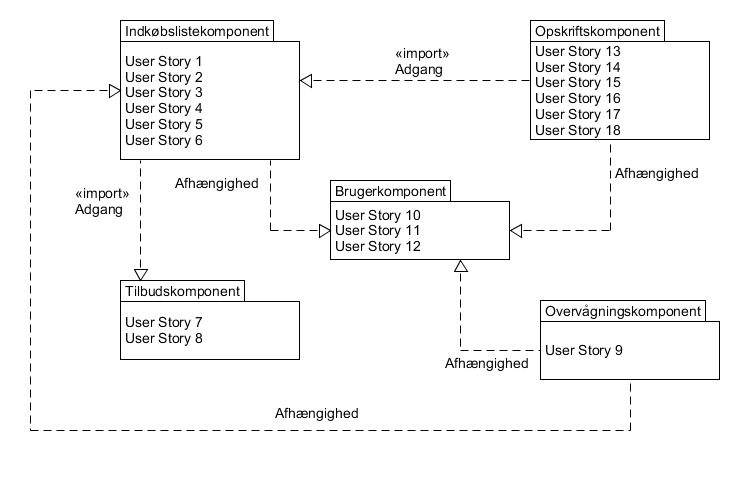
\includegraphics[width=1\textwidth]{images/Komponenter.png} % trim=1.4cm 6.1cm 6.5cm 1.8cm, clip, 
			\end{figure}
		\end{frame}

		\subsubsection{Modellag}
			\begin{frame}[t]{Arkitektur}\framesubtitle{Modellag}
				\begin{figure}
					
					\includegraphics<1-2>[trim=8.2cm 16.5cm 0.5cm 6.3cm, clip, width=1\textwidth]{images/PF_Model_UML_Simple.pdf} % ttrim=1.4cm 6.1cm 6.5cm 1.8cm, clip,
					\includegraphics<3>[width=0.5\textwidth]{images/UML_Pref_med_felter.png} % ttrim=1.4cm 6.1cm 6.5cm 1.8cm, clip,

				\end{figure}
				\begin{itemize}
					\item<2> Many-To-Many via bindeklasser med attributter
					\item<3> Problemer med modellaget
				\end{itemize}
			\end{frame}
		
		\subsection{Programmering}
			\begin{frame}{Programering}
				\begin{columns}
					\begin{column}{.48\textwidth}
						\begin{itemize}
							\item Git
							\begin{itemize}
								\item Branching
								\item Code-review
							\end{itemize}
							\item Pair Programming
							
						\end{itemize}

					\end{column}
					\begin{column}{.48\textwidth}
						\textbf{Branches:}
						\begin{itemize}
							\item master
							\item develop
							\item feature-xyz
							\item bugfix-abc
						\end{itemize}
					\end{column}
				\end{columns}
			\end{frame}


		\subsection{Teknologier}
			\begin{frame}[t]{Teknologier} %\framesubtitle{Udvikling intro}
				\begin{itemize}
					\item<1> ASP.NET
					\begin{itemize}
						\item<1> MVC
						\item<1> Razor view engine
						\item<1> Login system
					\end{itemize}
					\item<2> Entity Framework
					\begin{itemize}
						\item<2> Object--relational mapping
						\item<2> Code--first
						\item<2> Migrations
					\end{itemize}
					\item<3> Bootstrap
					\begin{itemize}
						\item<3> Responsiv layout
						\item<3> CSS--klasser og JS
					\end{itemize}
				\end{itemize}
			\end{frame}

		\subsection{eTilbudsavis API}
			\begin{frame}[t]{Teknologier} \framesubtitle{eTilbudsavis API}
			Kommunikation med API'en:
				\begin{enumerate}
					\item<1> POST api.etilbudsavis.dk/v2/\textbf{sessions}?api\_key=[...]
					\begin{itemize}
						\item<1> Modtag \texttt{token}
						\item<1> Beregn \texttt{signature} (SHA-256)
					\end{itemize}
					\item<2> GET api.etilbudsavis.dk/v2/\textbf{offers}?r\_lat=57\&r\_lng=9
					\begin{itemize}
						\item<2> Modtager 100 tilbud som JSON
						\item<2> Gentages til alle er modtaget (do..while)
						\item<2> Konverteres til \texttt{Offer}--klassen
					\end{itemize}
				\end{enumerate}
				\begin{itemize}
					\item<3> Er tidskrævende (60-300 sekunder)
					\item<3> Kan muligvis paralelliseres for bedre hastighed
					\item<3> Dataet kunne være bedre
				\end{itemize}
			\end{frame}
%\section{Program Demonstration}

\begin{frame}{Program demonstration}
	
	\begin{itemize}
		\item Database 
		\item Hvad sker der ved opstart?
		\item Hvad sker der når programmet lukkes?
	\end{itemize}

	
\end{frame}
%\input{slides/sass.tex}
\section{Refleksion og perspektivering}
\begin{frame}{Indhold}
  \begin{itemize}
    \item Konklusion
    \item Forbedringsforslag
    \item Udvidelse af systemet
  \end{itemize}
\end{frame}

\subsection{Konklusion}
\begin{frame}{Konklusion}
  \framesubtitle{Er problemformuleringen løst?}
  \[
  \left[
  \begin{minipage}{\textwidth}
  \centering
  \begin{minipage}{0.94\textwidth}
  \textit{Hvordan designes og implementeres et system, i C\#, der kan give brugere lettere adgang til dagligvarebutikkernes tilbud integreret med indkøbslister og opskrifter imens det gøres mere overskueligt, at handle ind til aftensmad?}
  \end{minipage} 
  \end{minipage}                           
    \right]
\]
\end{frame}
\begin{frame}{Konklusion}
  \framesubtitle{User stories og systemdefinition}
    \begin{itemize}
      \item User stories
      \begin{itemize}
        \item Acceptance
      \end{itemize}
      \item Systemdefinition
      \begin{itemize}
        \item \textit{.. anbefaler opskrifterne, baseret på bedømmelser .. og præferencer.}
      \end{itemize}      
    \end{itemize}
\end{frame}

\subsection{Forbedringsforslag}

\begin{frame}{Forbedringsforslag}
  \framesubtitle{Hvad kunne arbejdes videre på?}
  \textbf{Billeder}
  \begin{itemize}
    \item Opskrifter
    \item Tilbud
    \item General grafik
  \end{itemize}
\end{frame}

\begin{frame}{Forbedringsforslag}
  \framesubtitle{Hvad kunne arbejdes videre på?}
  \textbf{Indkøbslister}
  \begin{figure}
    \includegraphics<handout:1>[trim=0.2cm 0.2cm 0.2cm 2.2cm, clip, width=0.9\textwidth,height=0.8\textheight,keepaspectratio]{images/listenu.png}
     \includegraphics<handout:2>[trim=0.2cm 0.2cm 0.2cm 2.2cm, clip, width=0.9\textwidth,height=0.8\textheight,keepaspectratio]{images/listeny.png}
  \end{figure}
  
\end{frame}

\begin{frame}{Forbedringsforslag}
  \framesubtitle{Hvad kunne arbejdes videre på?}
  \textbf{Tilbud}

  \begin{figure}
    \includegraphics<1>[width=0.9\textwidth,height=0.8\textheight,keepaspectratio]{images/Screenshots/Offersmp.png}
  \end{figure}

\end{frame}


\begin{frame}[t]{Forbedringsforslag}
  \framesubtitle{Hvad kunne laves om?}
  \texttt{Nuværende API-data}
  \hbox{\hspace{5 mm}\scalebox{0.55}{
    \lstinputlisting{code/api/old.json}
  }
  }
\end{frame}

\begin{frame}[t]{Forbedringsforslag}
  \framesubtitle{Hvad kunne laves om?}
  \texttt{Forslag til præcisering af API-data}
  \hbox{\hspace{5 mm}\scalebox{0.55}{
    \lstinputlisting{code/api/new.json}
  }
  }
\end{frame}

\subsection{Programudvidelse}
\begin{frame}{Programudvidelse}
  \framesubtitle{Hvad kunne tilføjes?}
  \begin{itemize}
    \item Tøm køleskabet
    \item Normalpriser for alle varer
  \end{itemize}
\end{frame}

\section{Demonstration}
\begin{frame}{Indhold}
    \begin{itemize}
        \item Typisk workflow
        \item Implementering
        \item Mobil udgave 
        \begin{itemize}
	    	\item Indkøbslister
	    	\item Overvågningsliste
	    	\item Tilbud
	    	\item Opskrifter
        \end{itemize}   
    \end{itemize}
\end{frame}

\begin{frame}{Typisk workflow}
	\begin{itemize}
	\item Oprette bruger
	\item Bruge indkøbsliste og tilbud
	\item Finde opskrift og lave min egen
	\item Ændre mine præferencer
	\end{itemize}
	\href{http://james:8080}{Demonstration af ProjectFood}
\end{frame}

%%%% Implementering
\section{Implementering}
\begin{frame}{Indhold}
	\begin{itemize}
	\item Brugerens oplevelse
	\vspace{20pt}
	\item Model - Repræsentation af data
	\item Controller - Relevant logik
	\item View - Visualisering
	\end{itemize}	
\end{frame}

%% Model
\subsection{Model}
\begin{frame}{Model}
	\framesubtitle{Indkøbslister}
	\texttt{ShoppingList.cs}
	\lstinputlisting{code/model/ShoppingList.cs}	
\end{frame}
\begin{frame}{Model}
	\framesubtitle{Varer}	
	\texttt{Item.cs}
	\lstinputlisting{code/model/Item.cs}	
\end{frame}
\begin{frame}{Model}
	\framesubtitle{Overvågningsliste}
	\begin{itemize}
		\item Simpel implementering
		\item Specialiseret indkøbsliste
		\item Genkendes på titel  \texttt{\_watchList}
	\end{itemize}
\end{frame}
\begin{frame}{Model}
	\framesubtitle{Tilbud}
	\texttt{Offer.cs}
	\lstinputlisting{code/model/Offer.cs}	
\end{frame}
\begin{frame}{Model}
	\framesubtitle{Opskrifter}
	\texttt{Recipe.cs}
	\lstinputlisting{code/model/Recipe.cs}	
\end{frame}

%% Controller
\subsection{Controller}
\begin{frame}{Controller}
	\begin{itemize}
		\item CRUD - \texttt{Create()}, \texttt{Index()} og \texttt{Details()}, \texttt{Edit()}, \texttt{Delete()}
		\item \texttt{DataBaseContext} giver adgang til model-laget
		\vspace{15pt}
		\item Tilføje og fjerne varer, tilbud og ingredienser
		\item Kommunikation med API
		\item Information til brugere
	\end{itemize}
	%Indsæt relevant kode måske? eller tab til VS 
\end{frame}

%% View
\subsection{View}
\begin{frame}{View}
	\begin{itemize}
		\item Overblik - \texttt{Index.cshtml}
		\begin{itemize}
			\item \texttt{foreach} der ittererer over alle objekterne fx indkøbslister
		\end{itemize}
		\item Specifik objekter - \texttt{Details.cshtml}
		\begin{itemize}
			\item \texttt{foreach} der ittererer over eventuelle lister, som objektet har fx varer på en indkøbsliste
		\end{itemize}
		\item Razor tillader C\# i views
		\item Ajax, json og javascript
		\item Bootstrap modal, tabs og lignende
	\end{itemize}
\end{frame}

% ====================================================

% Final slide
{\aauwavesbg
  \begin{frame}[plain,noframenumbering]
    \finalpage{\texttt{throw new PresentationIsOverException();}}
  \end{frame}}

\end{document}
